% Auto-generated snippets for inclusion in the manuscript.

\begin{table}[t]
  \centering
  \caption{Neural Hawkes benchmark on Binance BTCUSDT (2025-09-21) and LOBSTER AAPL (2012-06-21). Metrics are reported on the test split. Lower is better for NLL/MAE/ECE; higher is better for accuracy and KS-$p$.}
  \label{tab:hawkes-benchmark}
  \begin{tabular}{l l r r r r r}
    \toprule
    Venue & Backbone & NLL $\downarrow$ & MAE [s] $\downarrow$ & Acc $\uparrow$ & KS-$p$ $\uparrow$ & ECE $\downarrow$ \\
    \midrule
    Binance & GRU         & 0.265 & 0.085 & 0.892 & $<10^{-6}$ & 0.035 \\
    Binance & Transformer & \textbf{0.252} & \textbf{0.083} & \textbf{0.898} & $<10^{-6}$ & 0.040 \\
    LOBSTER & GRU         & 4.512 & 0.974 & 0.858 & $<10^{-6}$ & 0.591 \\
    LOBSTER & Transformer & \textbf{4.425} & \textbf{0.899} & 0.858 & $<10^{-6}$ & 0.637 \\
    \bottomrule
  \end{tabular}
\end{table}

\begin{figure}[t]
  \centering
  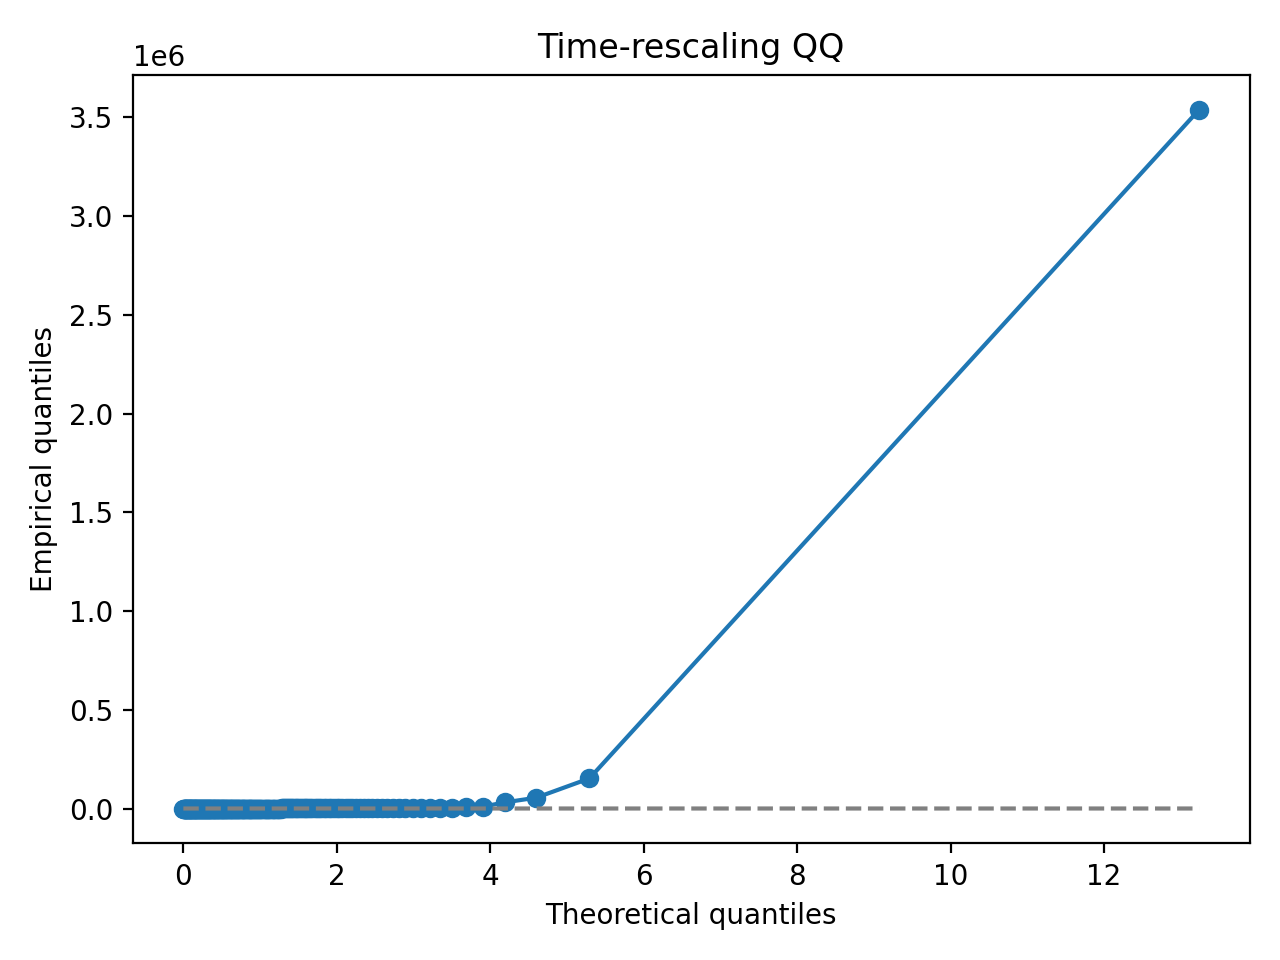
\includegraphics[width=0.32\linewidth]{figs/binance_transformer_long_qq_rescaled.png}
  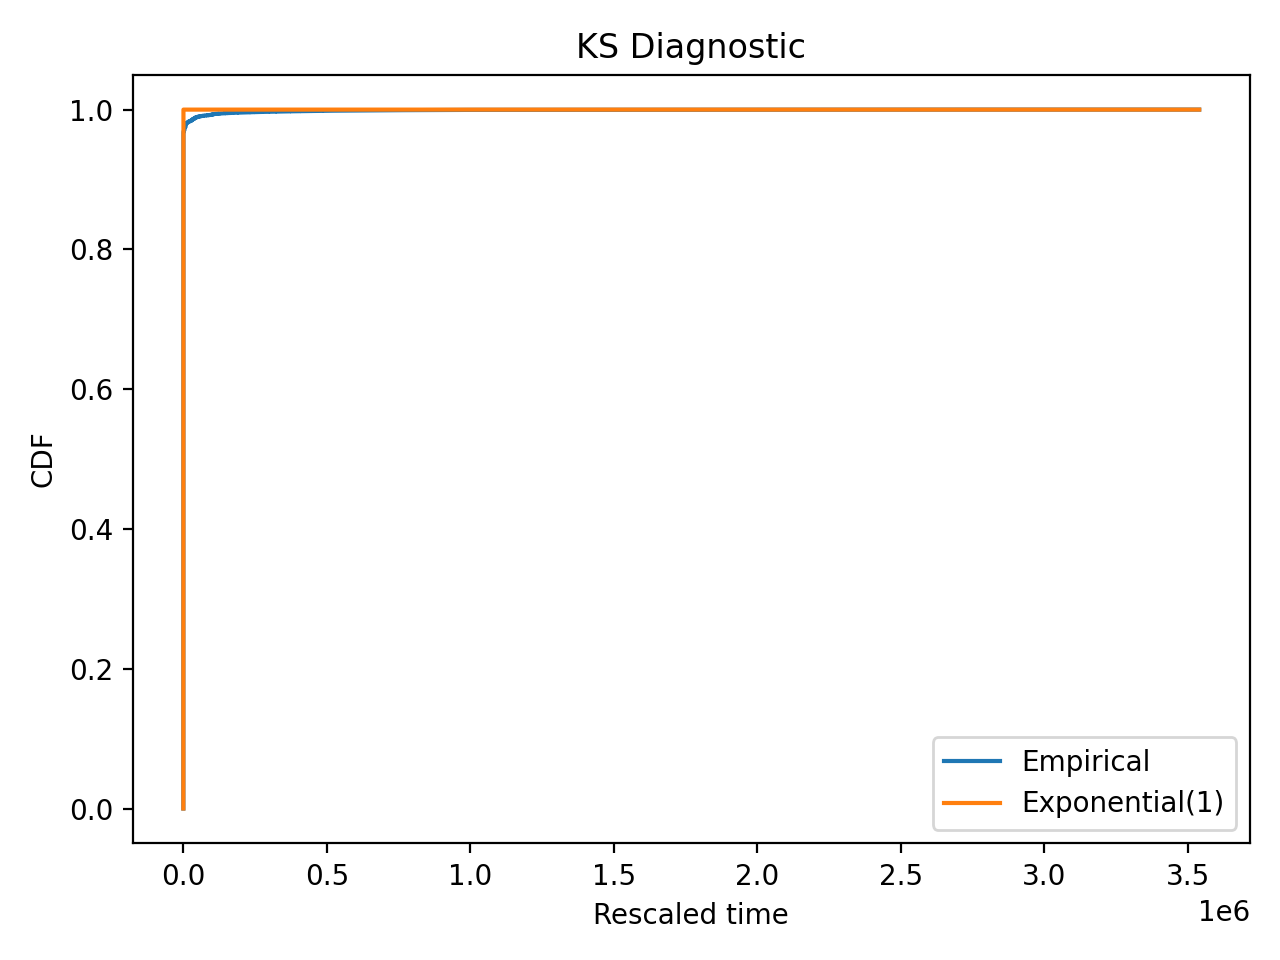
\includegraphics[width=0.32\linewidth]{figs/binance_transformer_long_ks_cdf.png}
  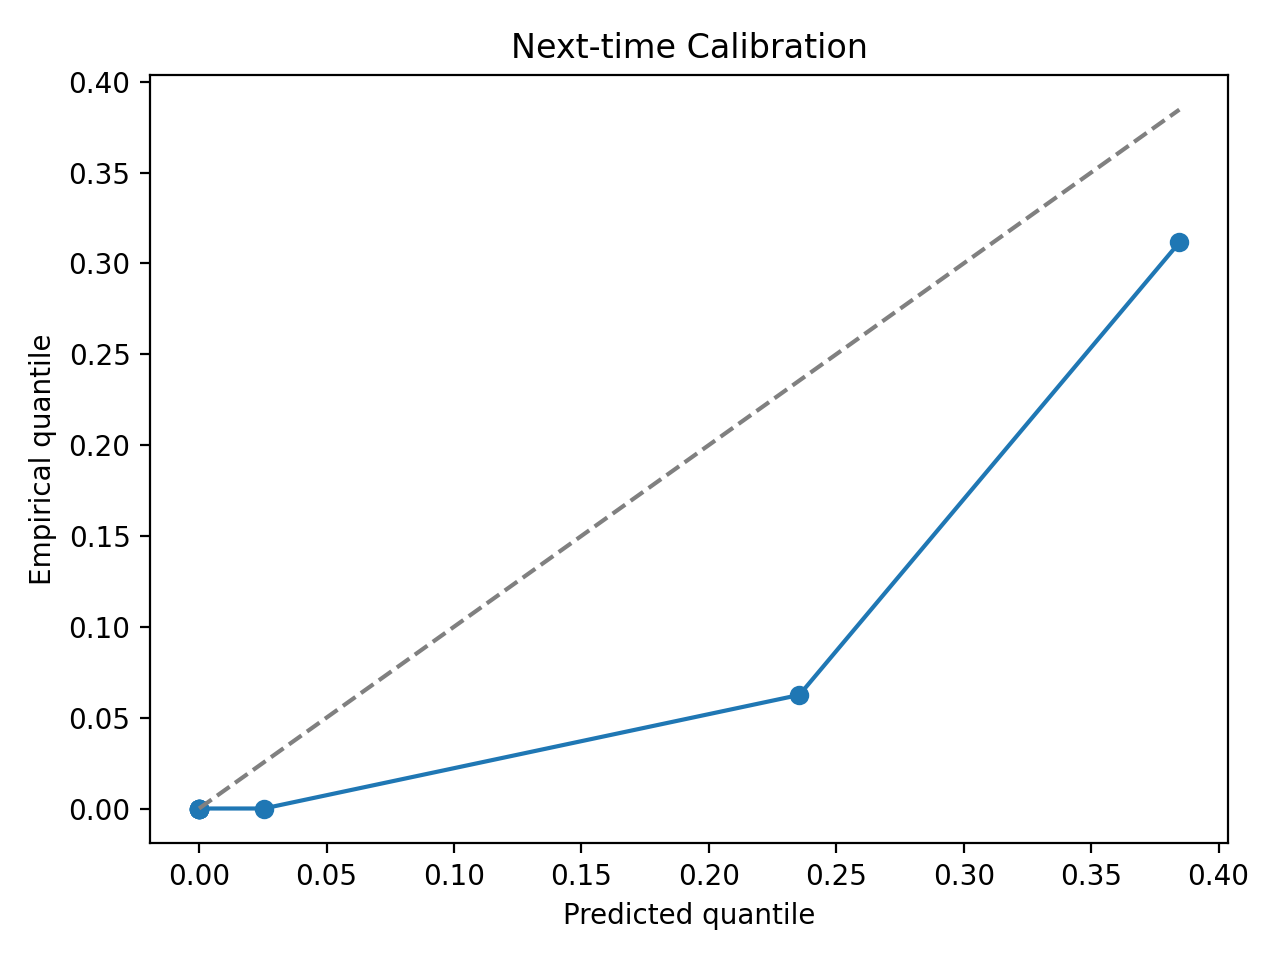
\includegraphics[width=0.32\linewidth]{figs/binance_transformer_long_calibration.png}
  \caption{Diagnostics for the Binance Transformer run: time-rescaling Q--Q plot, empirical vs. theoretical CDF (KS test), and next-arrival calibration curve. Ideal models would lie on the dashed diagonals.}
  \label{fig:hawkes-diagnostics}
\end{figure}

\paragraph{Empirical results.}
Replacing the GRU backbone with a transformer reduces NLL on Binance by $5.0\%$ (0.265$\rightarrow$0.252) and improves next-type accuracy from $0.892$ to $0.898$ while keeping the inter-arrival MAE comparable. On LOBSTER the transformer yields a milder $1.9\%$ NLL gain (4.51$\rightarrow$4.43) but trims the MAE by $0.075$ seconds. Despite these gains, both backbones fail the KS time-rescaling test (p-values $<10^{-6}$) and exhibit non-zero calibration error (ECE $\approx$0.04 on Binance, $\approx$0.63 on LOBSTER), motivating future work on explicit intensity calibration.

\appendix
\section*{Reproducibility checklist}
\begin{itemize}
  \item \textbf{Data.} Rebuild the NPZ datasets using
  \texttt{scripts/pack\_binance\_npz.py} (Binance BTCUSDT, day 2025-09-21) and
  \texttt{scripts/preprocess\_lobster.py} (LOBSTER AAPL, 2012-06-21). Metadata JSON files capture seeds and preprocessing flags.
  \item \textbf{Training.} Run
  \texttt{PYTHONPATH=. python experiments/run\_matrix.py --config experiments/configs/*\_backbones.json}
  for Binance and LOBSTER. Default seeds are 2024.
  \item \textbf{Diagnostics.} Execute
  \texttt{python scripts/collect\_runs.py} followed by
  \texttt{python scripts/prepare\_summary\_assets.py} to regenerate tables and figures.
  \item \textbf{Hardware.} Experiments were run on CPU (Apple M-series) and take 4--6 minutes per configuration.
\end{itemize}
